\documentclass[conference]{IEEEtran}

% for numbered citations
\usepackage{cite}
% for figures based on pdfs
\usepackage[pdftex]{graphicx}
 

\begin{document}
\title{Analyzing Parallel Programming Models for Analysis of Small Object Orbital Data}


% author names and affiliations
% use a multiple column layout for up to three different
% affiliations
\author{\IEEEauthorblockN{Kat Volk}
\IEEEauthorblockA{Lunar and Planetary Laboratory\\
University of Arizona\\
Tucson, Arizona\\
Email: kvolk@lpl.arizona.edu}
\and
\IEEEauthorblockN{Benjamin James Gaska, Neha Jothi, Mahdi Soltan Mohammadi, \\and Michelle Mills Strout}
\IEEEauthorblockA{Computer Science\\
University of Arizona\\
Tucson, Arizona\\
Email: \{bengaska, nehaj, mahdi.s.m.k, mstrout\}@email.arizona.edu}}

\maketitle

%%%%%%%%%%%%%%%%%%%%%%%%%%
\begin{abstract}
When new small objects are discovered in the Kuiper belt, a common first step is to simulate the orbits
of the observed objects forward in time and then analyze the simulation results to distinguish between 
various types of orbital evolution.  One key piece of information is whether the object is in an orbital resonance
with Neptune.  Currently this information us determined using analysis codes written
in Perl.  The problem is that the analysis experiences significant load imbalance and interpretation
overhead, both of which result in the analysis of the most time consuming objects requiring
about 15 minutes.  NASA's Large Synoptic Survey Telescope (LSST) will begin operations in the early to mid
2020's and is expected to discover and track $\sim$40K Kuiper belt objects over a ten year survey (compared to 
the $\sim1000$ currently known objects), so the need to do this analysis more efficiently is critical.
At 15 minutes for the time consuming cases (which we expect to be X\% of the discovered objects), the necessary 
once a month analyses would take over 3 months.
In this paper, we improve the execution time of the analysis by more than an order of 
magnitude.  We do this by porting the analysis to various programming languages:
parallel perl, Python, Chapel, Go, OpenMP, MPI, and Cilk++.
We compare these implementations in terms of performance, accuracy,
and maintainability from the perspective of the scientists.  We also
identify the key problems in this workload in terms of parallelization and
experiment with some possible parallelizations that help with the 
significant load imbalance.
\end{abstract}

\IEEEpeerreviewmaketitle

%%%%%%%%%%%%%%%%%%%%%%%%%%%
%\section{Questions}
%
%\begin{itemize}
%\item Who else is writing analysis codes for discovering orbital resonance and libration and
%what programming language are they using?
%People describe what analyses they are doing but not how they are coding it up and 
%software not typically shared. Publish results of such analyses.
%Typically Fortran is what is posted.
%Observational survey posting Fortran and Python code to github.
%Saw these objects, what are they doing?  Code for classifying might not be publically
%available due to support reasons.
%
%\item How much variance is there between objects that take require checking most of the
%ratios and those that require few checks?  What are some concrete numbers?
%Kat might be able to give us a distribution on this. (60\% ish)
%
%\item Can put into models about history of Neptune.
%
%\item What does it mean when we say that the classification has happened manually?
%Every single classification is still checked by an eye.  Could do a second check?
%
%\item Year that LSST should come online?  5 to 10 years from now.
%
%\item Do we only need to do the analysis for each object once?
%Everytime fit the orbit with new observations.  Whole sky once per month.
%\end{itemize}

%%%%%%%%%%%%%%%%%%%%%%%%%%
\section{Introduction}

Astronomers and planetary scientists would like to know which observed
objects in the Kuiper belt are in orbital resonance with Neptune. These
resonant objects are of particular interest because their distribution can
be used as an observational test for theoretical models of the 
outer Solar System's dynamical history \cite{Malhotra1993,Morby2008,Volk2016}.
%By characterizing such objects, the models of the history of Neptune
%can be fine tuned. 
The process by which such objects are currently being characterized
does not scale to the number of expected objects that the
upcoming Large Synoptic Survey Telescope (LSST) will enable scientists to find.
This paper describes the analysis workload, why the workload does not
scale, and presents and evaluates alternative implementations.

The classification process, which is detailed by \cite{Gladman2008}, entails the 
following basic steps:
(1) the position of the object in the sky at a variety of epochs is determined from observations 
(2) these positions are used to fit an orbit (a combination of position and velocity) for the observed object
(3) simulating the orbit forward in time under the gravitational influences of the Solar System's planets,
and
(4) analyzing the simulated orbit to determine if the object is
in resonance with Neptune.
If the object is in resonance with Neptune, then the analysis
program also determines which specific resonance the object is in
and the amplitude of libration for the associated resonance angle. 
The resonance angle describes the relative positions of the KBO and
Neptune when the KBO has its closest approach to the Sun; when an object's
evolution is controlled by the resonance, the angle will librate around a central
value, whereas objects not in resonance will have a resonance angle that freely
circulates between 0 and $360^{\circ}$. The resonance is labeled p:q according to the
period ratio between the object and Neptune; a 3:2 (p=3, q=2) resonance is one where 
the Kuiper belt object's orbital period is 1.5 times Neptune's orbital period. Figure~\ref{f:res-example}
shows the geometry us such a resonance.
%[Kat: I think we need a 2 column figure.  On the left a picture of 
%an object and Neptune orbiting the sun with a caption describing
%the resonance ratio.  On the right, showing the graph that the 
%analysis generates and pointing out the libration angle.]
\begin{figure} %[htbp]
   \centering
   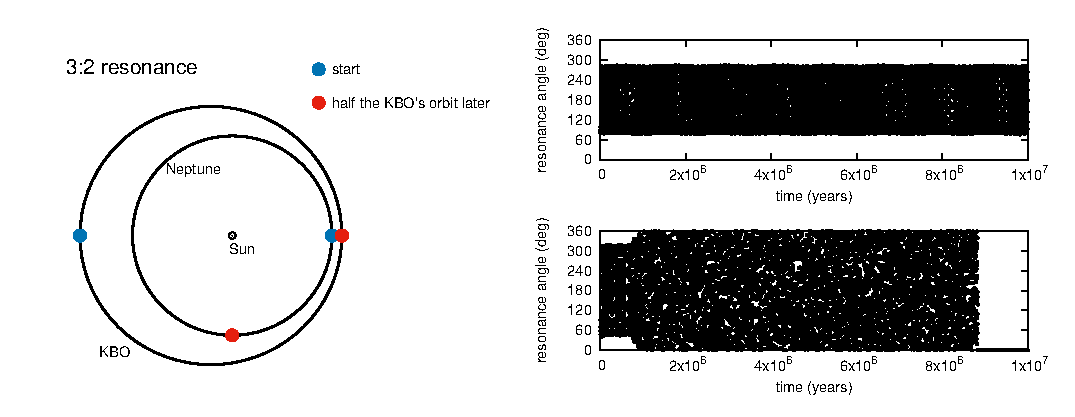
\includegraphics[width=6.2in]{multi-panel-res-figure.eps}
	\caption{Left: An illustration of the geometry of a 3:2 orbital resonance with Neptune. The Kuiper belt object's (KBO) orbital period is 1.5 times Neptune's orbital period; this means that while the KBO completes half an orbit, Neptune completes 3/4 of an orbit. Right: The resonance angle for an object in the 3:2 resonance (top) and one that starts in the resonance, but does not stay in resonance (bottom). }
   \label{f:res-example}
\end{figure}


The current performance bottleneck for this process is the
last step where the simulated orbit is analyzed for libration of any 
relevant resonance angles. A large number of p:q resonances must be
checked for each object, and objects that are near the correct period
ratio for a large set of p,q values take a long time to analyze.
To our knowledge, there is not a standard, open source code available to 
performs this analysis.  Researchers generally report
the results of such analyses in papers, but do not make their
codes available or report specific details about the analysis 
methodology [there's not really a citation to show this!].%~\cite{AnalysisResultsCitations}.
Therefore, we investigate the workload of a Perl script
that planetary scientist Dr. Kat Volk wrote to perform the analysis.

% NOTE: grouping the small, medium, and long term orbit analyses into one number.
The Perl code takes approximately 15 minutes on a Mac Mini to fully analyze an 
object that is close to many potential resonance ratios (some of these 
are eventually categorized as non-resonant).
It is not possible to determine up front whether a particle will pass
the initial resonance checks in seconds or require most of the 5 minutes
thus causing one level of load imbalance in the workload.
Typically 60\% [Kat: citation] of all observed particles require
the full analysis time.

With approximately
1000 objects in the last 20 years being classified as they are discovered in
groups of $\sim10-50$~\cite{Volk2016}, an analysis time
of up to 15 minutes per particle has not been an issue.
However, when the Large Synoptic Survey Telescope (LSST) comes 
online in the mid to late 2020's, the expectation is that forty thousand 
Kuiper belt objects will be discovered within the first few years of the survey
and will be continuously tracked over the survey's ten year lifespan.
Each month the LSST will scan the full southern sky multiple times and will provide new
measurements of the position of these objects.  Using the updated positions, the 
whole process of fitting a more accurate orbit and then 
analyzing the orbit for libration within a resonance will be redone
each month to provide more precise information for Kuiper belt researchers.
Unfortunately, with 60\% of the 10,000 objects requiring 15 minutes
each month, the analysis time for one month is currently over two months,
which clearly is a problem.
%10000*.60*15: 90000
%#/60: 1500
%#/24: 62.5
%Argument for speed
%\begin{verbatim}
%10000*5: 50000   ! number of objects times number of minutes for a long one. 
%#/60: 833.333333 
%#/24: 34.722222  ! number of days
%would really like to do this on 3 time scales, short, medium, and long term
%might want more precision with more stuff in time files
%\end{verbatim}

In this paper, we evaluate the process of porting the Perl analysis script
to Python, Chapel, Go, OpenMP, MPI, and Cilk++.
The ports were done in the context of a graduate course studying
parallel programming models.  We evaluate the ported programs
from the perspective of the programming language learning curve,
how realistic the language is for planetary scientists [Kat?],
the ease of use of the parallel constructs, and the performance.
We also show results comparing various parallelization strategies
for the code.

Although more room for improvement is possible and 
identified, some of the parallel versions we develop result in
an order of magnitude improvement.  The planetary scientists [Kat?]
will be able to use a parallel Python version that can do the
requisite analyses in just over 6 days, instead of 60 days.
The BLAH version was the fastest and would be able to do all
the analyses in XX days.



%%%%%%%%%%%%%%%%%%%%%%%%%%
\section{Methodology}

~\cite{ChapelOverviewJan13}


%%%%%%%%%%%%%%%%%%%%%%%%%%
\section{Conclusion}




%%%%%%%%%%%%%%%%%%%%%%%%%%
\section*{Acknowledgment}


%%%%%%%%%%%%%%%%%%%%%%%%%%
\bibliographystyle{IEEEtran}
\bibliography{libration.bib}

\end{document}


